\section{First approach}

Our first approach to design the system architecture was to develop:

\begin{itemize}
\item A software framework that
abstracted many common concepts found in different social networks (Facebook, Twitter, LinkedIn..)
like User, Post, Reply, Image and so on, to give the developers the possibility to use
(and extend) these abstractions seamlessly between different social networks.
\end{itemize}

\begin{itemize}
\item A java library to connect, using different mediums, to the Arduino devices in order
to send the data fetched from the social networks, and also a mechanism to manage Arduino's firmware,
to allow the device to support different configurations.
\end{itemize}

After the second meeting with the customer we decided to revise this plan, as this was not what
our customer really had in mind. Some of the code and documentation we produced earlier could be re-used, but some could not.

See appendix for more. \ref{app:firstdraftarchi}

\section{Revised approach}
The biggest difference in the new design is that API will still provide abstractions
for concepts common to the social network, but it will now focus on the estabilishing an interface,
using Android's Intent mechanism, between Social applications and the Bluetooth library.

\newpage
\section{Architecture diagram}
todo: bla bla ?
\begin{figure}[hb!]
\centering 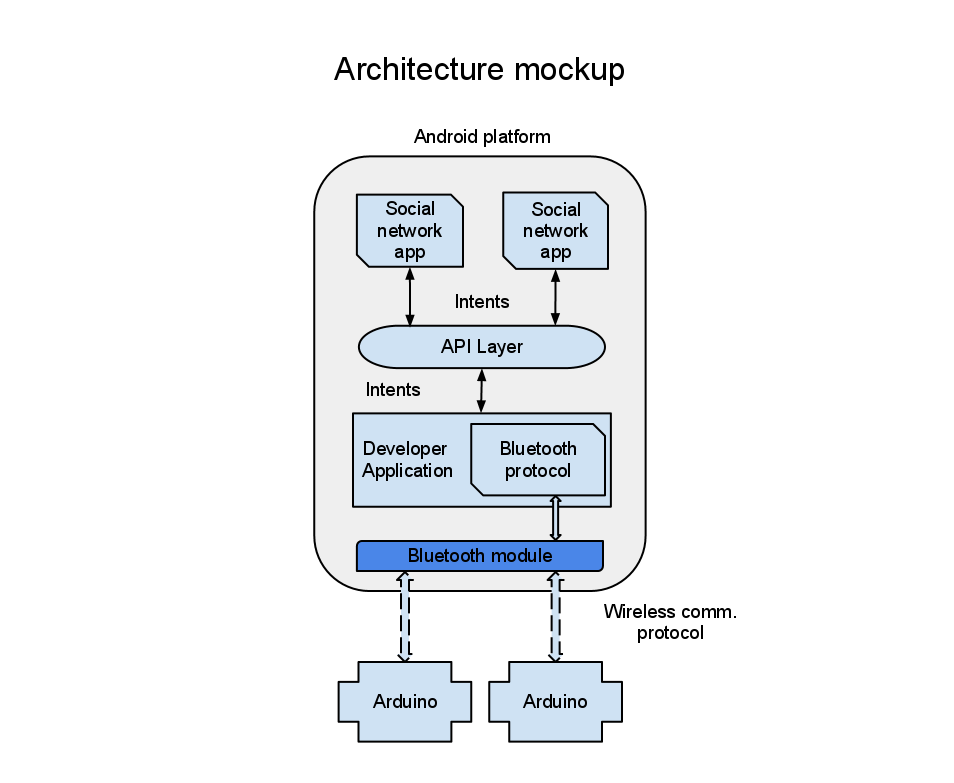
\includegraphics[scale=0.50]{img/architecture-diagram.png}
\caption{System architecture}
\label{fig:architecture}
\end{figure}

\newpage
\section{Use cases}
todo: bla bla?
\begin{figure}[hb!]
\centering 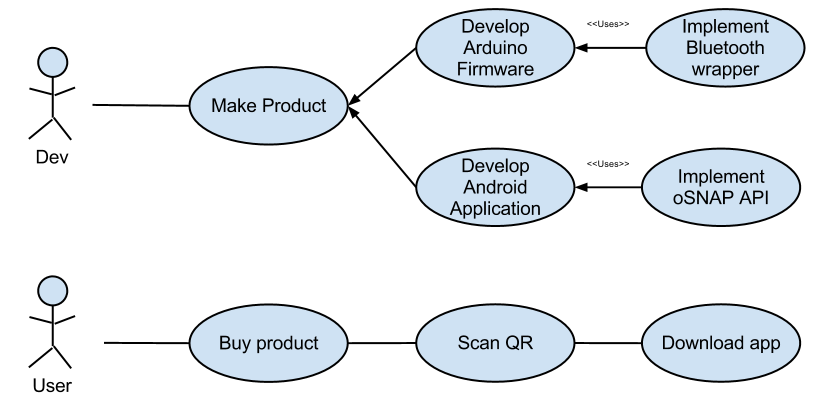
\includegraphics[scale=0.50]{img/use-cases.png}
\caption{Use cases}
\label{fig:architecture}
\end{figure}